\documentclass[11pt]{article}
\usepackage{setspace}
\usepackage[hidelinks]{hyperref}
\usepackage{url}
\usepackage[utf8]{inputenc}
\usepackage[english]{babel}
\usepackage[a4paper,top=2cm,bottom=2cm,left=2cm,right=2cm]{geometry}
\usepackage[T1]{fontenc}
\usepackage{graphicx}
\usepackage{longtable} %
\usepackage[caption = false]{subfig}
\usepackage{amsmath}
\usepackage{float}
\usepackage[style=authoryear,backend=biber]{biblatex}
\usepackage{lineno}
\usepackage{csquotes}% Recommended
\linespread{1.5}
\newcommand{\HRule}{\rule{\linewidth}{1mm}}
\addbibresource{references.bib}% Syntax for version >= 1.2
\usepackage{pgfgantt}

\begin{document}
% title
\title{Mechanistic Modelling of COVID-19 and Climate}%
\author{Ruth Keane}

\begin{titlepage}
\includegraphics[width=8cm]{logo.eps}\\[1cm] 
\center 
\textsc{\LARGE Project Proposal}\\[1.5cm] 
\textsc{\Large Imperial College London}\\[0.5cm]
\textsc{\large Life Sciences}\\[0.5cm] 
\makeatletter
\HRule \\[0.4cm]
{ \huge \bfseries \@title}\\[0.4cm] % Title of your document
\HRule \\[1.5cm]

\begin{minipage}{0.4\textwidth}
\begin{flushleft} \large
\emph{Author:}\\
\@author % Your name
\end{flushleft}
\end{minipage}
~
\begin{minipage}{0.4\textwidth}
\begin{flushright} \large
\emph{Supervisors:} \\
Dr Samraat Pawar \\[1.2em] % Supervisor's Name
Dr Michael Tristem\\[1.2em]
\end{flushright}
\end{minipage}\\[2cm]
\makeatother

{\large \today}\\[2cm] % Date, change the \today to a set date if you want to be precise0
\vfill % Fill the rest of the page with whitespace
\clearpage
\end{titlepage}

\linenumbers
\section{Keywords} % six needed
{\bf Keywords:} Temperature, Humidity, COVID-19, Mechanistic, SEIR model, Virology
\section{Introduction to Project Idea and Proposed Questions}
The current  pandemic of COVID-19 is the biggest health crisis humans have faced in the last century. It is caused by a novel coronavirus (SARS-CoV-2), first detected in Wuhan, Hubei, China which spread rapidly (\cite{WorldHealthOrganizationWHO2020Novel1}). Understanding what affects disease spread allows us to make predictions about where might be badly effected and prepare adequately.  \\
Climatic variables have been shown to affect virus transmission, for example in influenza (\cite{Lofgren2007InfluenzaTheories}) and hand-foot-mouth disease (\cite{Feng2014TimePredictors}). Influenza is seasonal, peaking in Winter in temperate countries, and does better in cold and wet conditions (\cite{Deyle2016GlobalInfluenza}).
This could be due to changes in human immunity%may be reduced at lower temperatures,
, human behaviour %that cause spread of viruses may differ between seasons (for example relating to school holidays)
 and virus stability (\cite{Lipsitch2009InfluenzaFog}).%may be different in different environments . 
  Experimental evidence has found transmission of influenza between guinea pigs in controlled environments depends on temperature and humidity (\cite{Lowen2007InfluenzaTemperature}). 
%so viral stability is very likely to contribute to influenza seasonality 
\\
Recent studies currently in preprint have explored whether SARS-CoV-2 also varies with climate. Experimentally,  SARS-CoV-2 has been found to be more stable at lower temperatures (\cite{Chin2020StabilityConditions}). 
%Some attempts have been made to use maximum entropy techniques to explore whether certain parts of the world are likely to be more susceptible to COVID-19 epidemics (\cite{Araujo2020SpreadClimate,Bariotakis2020ClimaticSARS-CoV-2}) but these approaches have been highly criticised (\cite{Chipperfield2017OnNaimi}).
Many studies have used phenomenological models (mostly linear models, including LOESS regressions and GLMs) to find links between climate and COVID-19 incidence or mortality (\cite{Wang2020HighCOVID-19,Luo2020TheOutbreak,Sajadi2020TemperatureCOVID-19,Bannister-Tyrrell2020Preliminary2020,Rahman2020AOutbreak,Oliveiros2020RoleCases,Chen2020RolesScale,Ma2020EffectsWuhan,Poirier2020TheScales.}).  While limited by the quality of their data, most of these studies suggest that lower temperature and humidity increase SARS-CoV-2 transmission. An attempt to mechanistically model COVID-19 including temperature has been made (\cite{Shi2020TheChina}). In this work, an SEIR model was combined with a linear model representing the time-dependent rate of infectious contact, including temperature and absolute humidity as variables.
\\
The current work aims to mechanistically model the spread of COVID-19 using an SEIR model incorporating climatic variables (temperature and humidity) and use this to make predictions. This project will be more mechanistic than previous work and have access data with more spatial and temporal detail.\\
The main question being addressed is: To what extent is COVID-19 spread likely to depend on temperature and climate? Between region differences can be described (what locations are more at risk?). In addition, the effect of within region changes in climate would be useful to inform planning for individual countries (is COVID-19 likely get worse over winter in temperate countries?). Factors other than climate are likely to affect COVID-19 so understanding how these interact with climate is important (How does the effect of climate change at different levels of social interaction?).
\section{Proposed Methods}
This project will make an SEIR model for COVID-19. This will include modelling the survival of SARS-CoV-2 in different climatic conditions using experimental data about the survival coronaviruses outside of the host. Data is available for the change in viral titre over time at a range of temperatures and humidities for different coronaviruses (\cite{Lai2005SurvivalCoronavirus,Chin2020StabilityConditions,vanDoremalen2013StabilityConditions,Pyankov2018SurvivalAir,Casanova2010EffectsSurfaces}). These data sources could be combined, to produce a "survivability" function, perhaps outputting a percentage of the maximum possible survival. This will modify the probability of infection given contact between an infected and susceptible person (part of $\beta$ in the SEIR model). In addition, variation in human movement could be modelled, which would modify the contact rate component of $\beta$, improving our understanding of the interaction between climate and movement in the severity of the epidemic. COVID-19 case data will be used to estimate other parameters such as recovery rate. Sensitivity analysis will be carried out to understand how robust the model is to changes in parameters. This model will be used to make predictions about how the disease will spread over time. If time allows, we may attempt to validate the model with data.
\section{Anticipated Outputs and Outcomes}
The main outcome will be an SEIR model for COVID-19 which will be used to gain an understanding of how climate affects the spread of COVID-19 and how this interacts with human movement. Another outcome will be predictions about winter and potentially the future of COVID-19.
\section{Project Feasibility}
\vspace{-0.5cm}
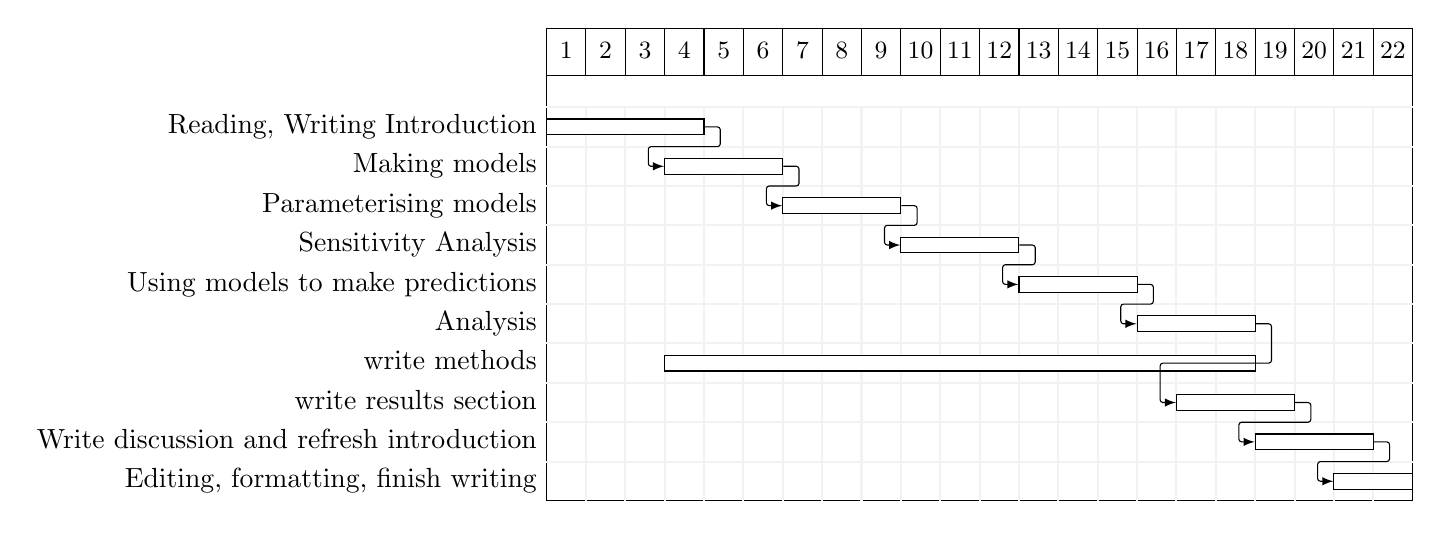
\begin{tikzpicture}[/pgfgantt/y unit chart=0.5cm]  
\begin{ganttchart}[hgrid={*1{draw=black!5, line width=.75pt}},vgrid={*1{draw=black!5, line width=.75pt}},title top shift=0]{1}{22}
  \gantttitlelist{1,...,22}{1} \\
  \ganttbar{Reading, Writing Introduction}{1}{4} \\
  \ganttbar{Making models}{4}{6}\\
  \ganttbar{Parameterising models}{7}{9}\\
  \ganttbar{Sensitivity Analysis}{10}{12}\\  
  \ganttbar{Using models to make predictions}{13}{15}\\
  \ganttbar{Analysis}{16}{18}\\
  \ganttbar{write methods}{4}{18}\\
  \ganttbar{write results section}{17}{19}\\
  \ganttbar{Write discussion and refresh introduction}{19}{21}\\
  \ganttbar{Editing, formatting, finish writing}{21}{22}
  \ganttlink{elem0}{elem1}
\ganttlink{elem1}{elem2}
\ganttlink{elem2}{elem3}
  \ganttlink{elem3}{elem4}
\ganttlink{elem4}{elem5}
\ganttlink{elem5}{elem7}
  \ganttlink{elem7}{elem8}
\ganttlink{elem8}{elem9}
\end{ganttchart}
\end{tikzpicture}
\vspace{-1.5cm}
\section{Itemized Budget}
Computer improvements -£200- Additional RAM (if needed), possibly a monitor, hard drive \\
Books- £100- May need to be purchased due to lack of library (if essential and not available online)

\clearpage{}
\printbibliography

\clearpage{}
\section*{Budget Approval}
\textbf{I have seen and approve the proposal budget} \\
Name: Samraat Pawar \\
Signature: \\
Date:
\end{document}